\documentclass[tikz]{standalone}
\usepackage[T1]{fontenc}
\usepackage[utf8]{inputenc}
\usepackage{pgfplots}
\usepackage{grffile}
\pgfplotsset{compat=newest}
\usetikzlibrary{plotmarks}
\usetikzlibrary{arrows.meta}
\usepgfplotslibrary{patchplots}
\usepackage{amsmath}

\begin{document}
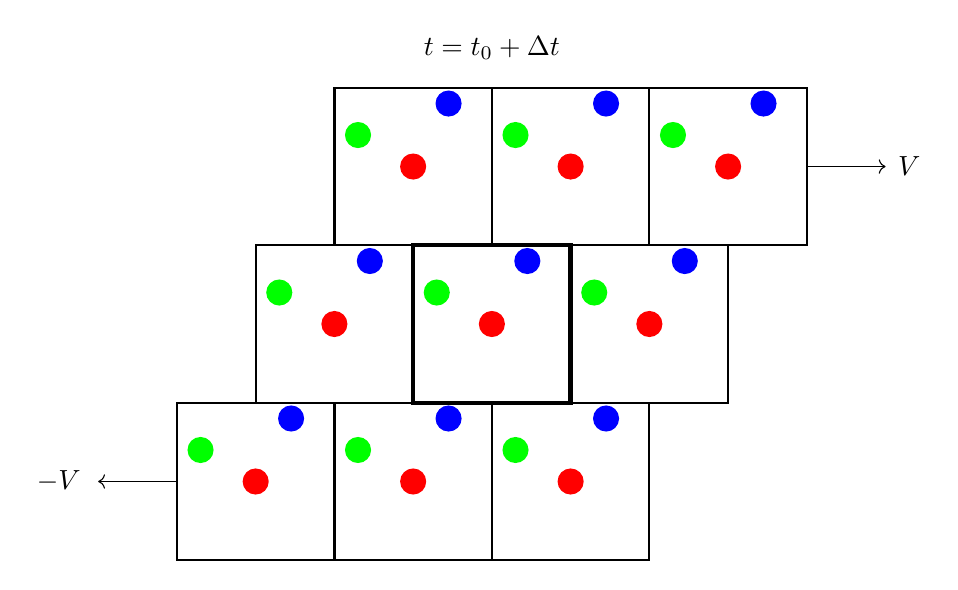
\begin{tikzpicture}


\foreach \x in {5,7,9} {
    \foreach \y in {1,3,5} {
        \node[circle, fill=blue] at (\x+\y/2+0.45+1,\y+1.8) {};
        \node[circle, fill=green] at (\x+\y/2+0.3 ,\y+1.4) {};
        \node[circle, fill=red] at (\x+\y/2+1 ,\y+1) {};
        
        % edge of each box
        \path[draw,thick] (\x+\y/2,\y) rectangle (\x+\y/2+2,\y+2);
    }
}


\path[draw,ultra thick] (8.5,3) rectangle (10.5,5);
 \draw[->](5.5,2)--(4.5,2);
  \draw(4,2)node{$-V$};
  
 \draw[->](13.5,6)--(14.5,6);
  \draw(14.8,6)node{$V$};
  
  \draw(9.5,7.5)node{$t=t_0+\Delta t$};
\end{tikzpicture}%
\end{document}